\section{A Generative Story for Leaderboards}
\label{ch:isicle:lead}

\begin{figure}[t]
  \centering
  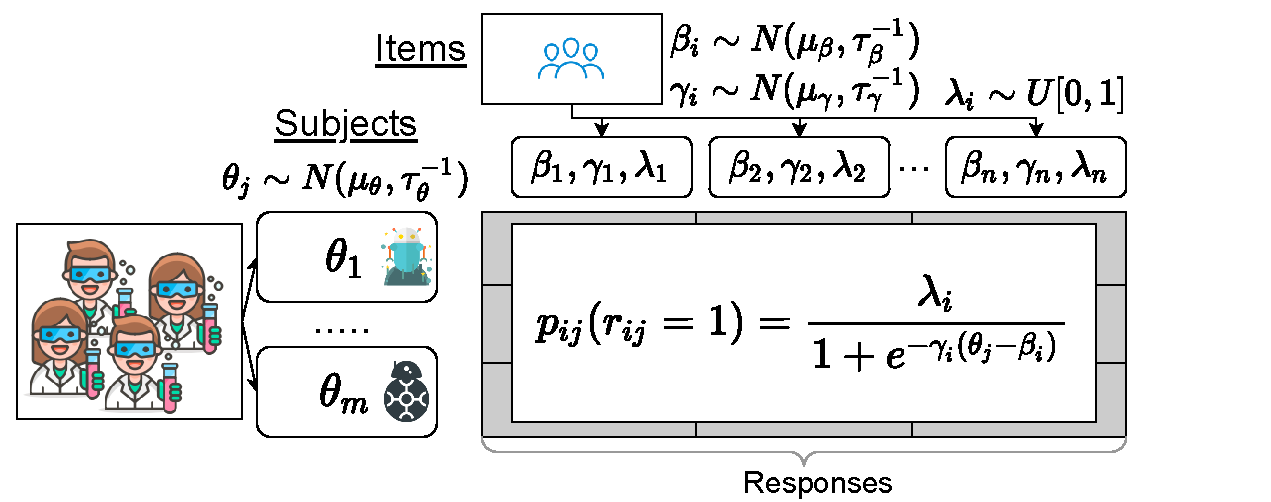
\includegraphics[width=.97\columnwidth, trim=0.5cm 0.3cm 2.6cm .4cm]{leaderboard}
  \caption{
    A \name{} leaderboard uses \irt{} to jointly infer \itm{} \diff{} $\beta_i$, \discability{} $\gamma_i$, feasibility~$\lambda_i$, and \subj{} skill $\theta_j$.
    These predict the likelihood $p_{ij}(r_{ij}=1)$ of a correct response $r_{ij}$.
  }
  \label{fig:story}
\end{figure}

Leaderboards are a product of the metrics, evaluation data, and
\subj{}s (machine or human) who answer \itms{}
(Figure~\ref{fig:story}).
For concreteness, let's assume that we have a question-answering task and two \subj{}s: \smart{},
who is good at trivia, and \dumb{}, who is not.
In the simplest \irt{} models, each \subj{}~$j$ has a random
variable~$\theta_j$ corresponding to their skill: \smart{}'s is big,
\dumb{}'s is small.

But you cannot know that until you start asking them questions of
varying \iemph{difficulty}~$\beta_i$.
Harder questions have a higher difficulty (``what is the airspeed of
an unladen swallow'') than easy ones (``who is buried in Grant's
tomb'').
The bigger the margin between a \subj{}'s skill~$\theta_j$ and an \itm{}'s
difficulty~$\beta_i$, $\theta_j-\beta_i$, the more likely that \subj{}~$j$
responds correctly~$p_{i,j}(r_{i,j}=1)$.
This is the simplest \abr{irt} model, which we call {\bf \pl{1}}.

Generally, given $n$ test items $\mathcal{X}=(X_1,\ldots,X_n)$
and $m$ \subj{}s
$\mathcal{S}=(S_1,\ldots,S_m)$, where each \subj{} answers every
item, we want to estimate \subj{} skills and \itm{} difficulties.
To discover the random variables that best explain the data, we
turn to probabilistic inference~\cite{pearl-88}.


Two additional random variables further improve \name{}:
\discability{} $\gamma_i$ and feasibility $\lambda_i$.
We first consider \discability{} and the margin between a
question's difficulty~$\beta_i$ and a \subj{}'s skill~$\theta_j$.
A discriminative question is challenging but can still be answered
correctly by a strong \subj{}.
If \smart{}'s ability is higher than most \itms{}' difficulty
($\theta_j-\beta_i$ is large), \itm{} discriminability multiplies this
gap by $\gamma_i$ in a model called {\bf \pl{2}}.
Questions with low $\gamma_i$ are low quality: they have annotation
error or do not make sense.

Another way of capturing poor quality questions is the
feasibility~$\lambda_i$.
For example, if the question ``who was the first president'' has the
answer \answer{Rajendra Prasad}, the question has an unstated implicit
assumption that \subjs{} must guess what country or company the
question is about.
In the model {\bf \pl{3}}, if a large fraction of \subj{}s all get an
\itm{} wrong, everyone's probability of getting the \itm{} right is
capped at $\lambda_i$.
In \nlp{} terms, $1-\lambda_i$ corresponds to the prevalence of annotation
errors that lead to unsolvable \itm{}s.


Having introduced all of the constituent elements of the model, we can
now present the full generative model:
\begin{enumerate*}
  \item For each subject $j$:
  \begin{enumerate*}
    \item Draw skill $\theta_j \sim \mathcal{N}(\mu_\theta, \tau_\theta^{-1})$
  \end{enumerate*}
  \item For each item $i$:
  \begin{enumerate*}
    \item Draw difficulty $\beta_i \sim\mathcal{N}(\mu_\beta, \tau_\beta^{-1})$
    \item Draw discriminability $\gamma_i \sim \mathcal{N}(\mu_\gamma, \tau_\gamma^{-1})$
    \item Draw feasibility $\lambda_i \sim \text{U}[0,1]$
  \end{enumerate*}
  \item Draw subject $i$ response on item $j$,\\$r_{ij} \sim p_{ij}(r_{ij} \mid \theta_j, \beta_i, \lambda_i )=$
    \begin{equation}
      p_{ij}(r_{ij}=1|\theta_j)=\frac{\lambda_i}{1+e^{-\gamma_i(\theta_j-\beta_i)}}.
      \label{eq:isicle:ours}
    \end{equation}
    For \pl{1}, $\gamma_i$ and $\lambda_i$ are fixed to 1.0, while for
    \pl{2}, only $\lambda_i$ is fixed.\footnote{In psychometrics, \pl{1}~is called a Rasch~\citep{rasch1960studies} or 1 parameter logistic (1PL) model, \pl{2}~is a 2PL model, and \pl{3}~is a 4PL model with guessing set to zero.}
\end{enumerate*}
Means $\mu_\theta,\mu_\beta,\mu_\gamma$ are drawn from
$\mathcal{N}(0,10^6)$ and $\tau_\theta,\tau_\beta,\tau_\gamma$
from a $\Gamma(1,1)$ prior, as in \citet{lalor2019latent} and
recommended by \citet{natesan2016birt}.\footnote{We differ by
  allowing $\gamma<0$ to identify bad \itms{}.  }

Because it is difficult to completely codify skill and difficulty into
a single number, we can rewrite the exponent in
Equation~\ref{eq:isicle:ours} as a sum over dimensions
$-\gamma_i(\sum_k \bm{\theta}_{j,k}-\bm{\beta}_{i,k})$,
where each dimension captures the interaction between an \itm{}'s
difficulty and a \subj{}'s skill.
For example, perhaps \dumb{} could better exploit artifacts in one
dimension (their skill for $\theta_{j,k=5}$ is high but everywhere
else is low) while \smart{} might not know much about a particular
topic like potent potables ($\theta_{j,k=2}$ is low but everywhere
else is high).
We call this model {\bf \pl{m}}.\footnote{
  We do not incorporate feasibility into the \pl{m}~model since it already improves over 1D models without it.
}
Multidimensional \irt{} models~\citep{reckase2009mirt} could---in addition to better modeling
difficulty---also cluster items for interpretation; we briefly
experiment with this (Appendix~\ref{ch:isicle:clustering}), but leave
more to future work (\S\ref{ch:isicle:future}).

\subsection{Examples are Not Equally Useful}

\irt{}'s fundamental assumption is that not all \itms{} and
\subjs{} are equal.
This explains why leaderboards can fail while having
``normal looking'' accuracies.
As a thought experiment, consider a dataset that is one third easy
($\beta_i \in [0,1]$), one third medium difficulty
($\beta_i \in [2,3]$), and one third hard ($\beta_i \in [6,7]$).
Suppose that \smart{} has skill $\theta_{k}=4$ while \dumb{} has skill
$\theta_{b}= 2$.
A standard leaderboard would say that \smart{} has higher accuracy
than \dumb{}.
But suppose there's a new \subj{} that wants to challenge \smart{};
they are not going to reliably dethrone \smart{} until their skill
$\theta_{c}$ is greater than six.

This is a more mathematical formulation of the ``easy'' and ``hard''
dataset splits in question
answering~\citep{sugawara2018easier,Rondeau2018-um,sen2020learn}.
In \pl{3}, this recapitulates the observation of
\citet{boydgraber2020nerds} that annotation error can hinder effective
leaderboards.
\name{} helps systematize these observations and diagnose dataset issues.


\subsection{Inference}

To estimate the latent parameters of our model, we use mean-field
variational inference~\cite{jordan-99}.
In variational inference, we propose a distribution over the latent
variables,~$q_\phi(\cdot)$, that approximates the true but intractable
posterior~$p(\cdot)$.
We then minimize the \abr{kl}-divergence between these distributions,
equivalent to maximizing the evidence lower-bound (\textsc{elbo}) with
respect to the variational parameters.

In our case, $q_\phi(\cdot)$ is a mean-field distribution, which means it
factorizes over each of the latent variables (the product is over the
$n \times m$ subject-item pairs)
\begin{align*}
  q_\phi(\bm{\theta}, \bm{\beta}, \bm{\gamma}, \bm{\mu}, \bm{\tau}) = q(\bm{\mu})q(\bm{\tau})\prod_{i,j} q(\theta_j)q(\beta_i)q(\gamma_i)
\end{align*}
Specifically, for our key latent variables $z \in \{\bm{\theta}, \bm{\beta}, \bm{\gamma}\}$, the associated variational distributions are of the form $q(z) = \mathcal{N}(u_z, t_z^{-1})$.
Recall that in the generative distribution, each latent $z$ is drawn from a $\mathcal{N}(\mu_z, \tau_z^{-1})$ whose parameters are also latent variables; for these variables, we use the variational distributions $q(\mu_z) = \mathcal{N}(u_{\mu_z}, t_{\mu_z}^{-1})$ and $q(\tau_z) = \Gamma(a_{\tau_z}, b_{\tau_z})$. We optimize the \textsc{elbo} with respect to the variational parameters
\begin{align*}
  \bm{\phi} & =\{\bm{u}_z,\bm{t}_z,\bm{u}_{\mu_z},\bm{t}_{\mu_z},\bm{a}_{\tau_z},\bm{b}_{\tau_z},\bm{\lambda}\}
\end{align*}
for all $z$ using \abr{adam}~\citep{Kingma2014AdamAM}.

With \name{}'s leaderboard \irt{} model introduced, we next discuss
how leaderboard \subj{}s are statistically compared and alternative
methods---such as using \irt{} parameters---to evaluate whether two
models are truly different.
